\documentclass[a4paper,twoside,14pt,hidelinks]{extarticle}


% Packages
% ---------------------

\usepackage{fancyhdr} % Head and foot options
\usepackage{hyperref} % Uses automatic references \autoref
\usepackage{titletoc} % Style table of contents with dots
\usepackage[T1]{fontenc}
\usepackage{libertine}
\usepackage[libertine]{newtxmath} % Font
\usepackage{graphicx} % Show images
\usepackage{natbib} % Bibliography
\usepackage{bm} % Make math bold with $\bm{some math}$
\usepackage{enumitem} % Customizable lists https://tex.stackexchange.com/a/42907/101976


% Typography
% ---------------------

% Page margins
\usepackage[top=2cm, bottom=2.5cm, left=2.5cm, right=2.5cm]{geometry}

% First line indentation
\setlength{\parindent}{2em}

% Line spacing
\renewcommand{\baselinestretch}{1.1}

% Color the links and references
\hypersetup{
    colorlinks=true, linkcolor=blue, filecolor=magenta, urlcolor=blue, citecolor=blue
}

\renewcommand{\UrlFont}{\small}

% Change spacing before and after titles {<left>}{<before-sep>}{<after-sep>}
% spacing: how to read {12pt plus 4pt minus 2pt}
%          12pt is what we would like the spacing to be
%          plus 4pt means that TeX can stretch it by at most 4pt
%          minus 2pt means that TeX can shrink it by at most 2pt
% https://tex.stackexchange.com/a/53341
\usepackage{titlesec}
\titlespacing*{\section}{0pt}{4em plus 2em minus 2em}{2em plus 1em minus 1em}
\titlespacing*{\subsection}{0pt}{2em plus 1em minus 1em}{1em plus .5em minus .5em}

% Precent stretching content vertically and adding empty space
\raggedbottom

% Remove numbers from sections
\setcounter{secnumdepth}{0}

% Set margins for the contents
\dottedcontents{part}[0em]{\bfseries}{0em}{1pc} % Use dots in the table of contents
\dottedcontents{section}[2em]{\bfseries}{2em}{1pc} % Use dots in the table of contents
\dottedcontents{subsection}[3em]{}{2em}{1pc} % Use dots in the table of contents


% Adjust spacing between apragraphs
% https://tex.stackexchange.com/a/375896
\setlength\parskip{1em plus 0.1em minus 0.2em}
\setlength\parindent{0pt}

% Title page
% ----------

\title{\normalsize ASP5020: Data analysis and machine learning \\\vspace{0.5cm}\Large Problem Set 5}
\author{\normalsize Evgenii Neumerzhitckii\\\normalsize Student ID: 27889076\vspace{0.3cm}}
\date{\normalsize Due: May 28, 2021\\\normalsize Submitted: May 29, 2021}

\begin{document}

\maketitle
\thispagestyle{empty} % Remove page number from title page

\vspace{0.5cm} % Add space between the title and table of contents
\tableofcontents
\thispagestyle{empty} % Remove page number from title page
\pagebreak


% Header and footer
% ---------------------

\pagestyle{fancy}
\fancyhf{}
\fancyhead[C]{Problem set 5}
\fancyhead[LE,RO]{\thepage}


% Parts
% ---------------------

\section{Question 1}

The data are shown on \autoref{q1_two_observations}.

\begin{figure}[!ht]
  \centering
  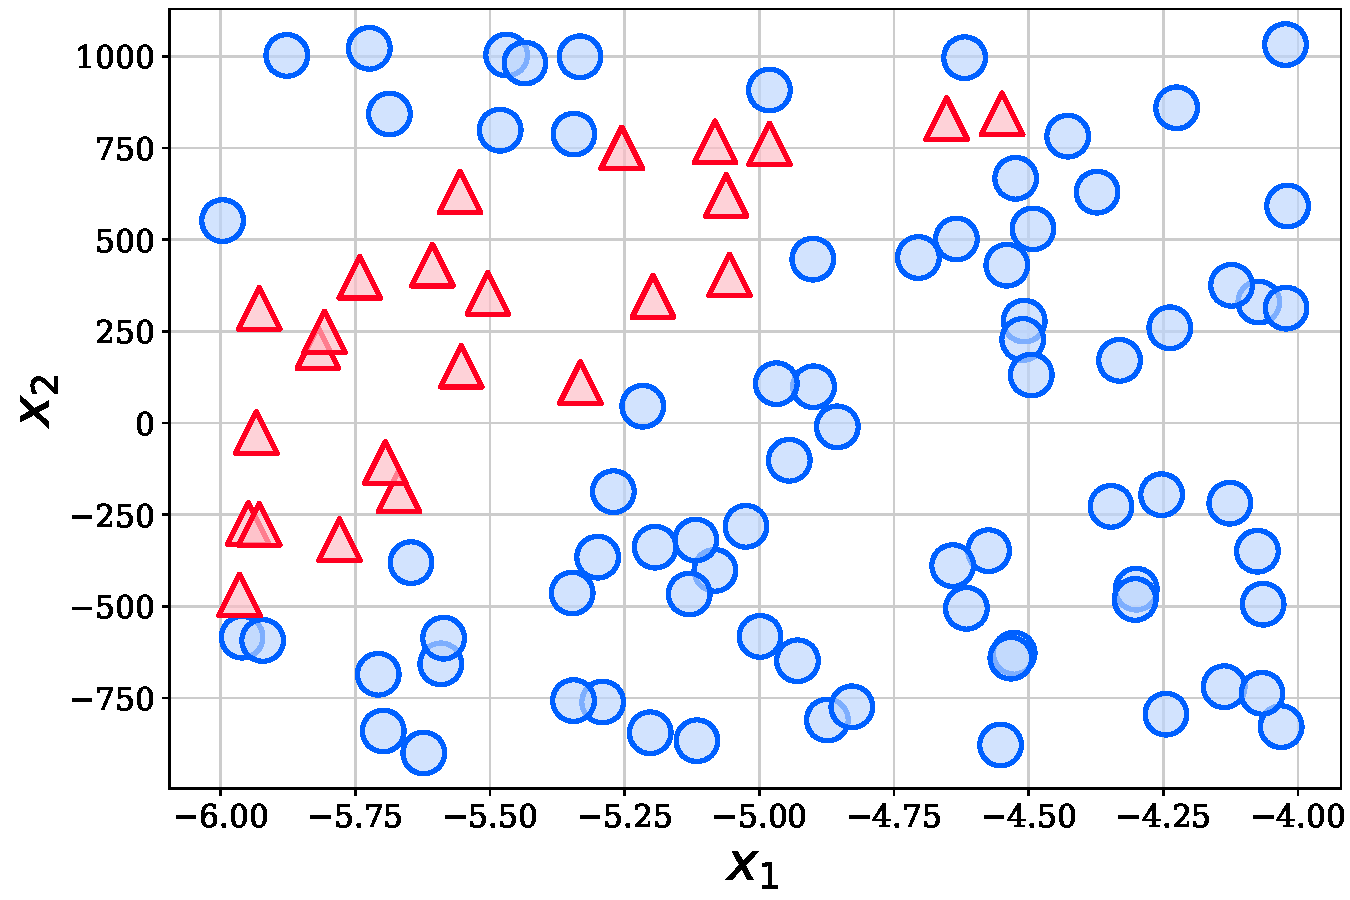
\includegraphics[width=0.8\textwidth]{figures/q1.pdf}
  \caption{Two types of observations. Code: q1.py.}
  \label{q1_two_observations}
\end{figure}

The diagram of the neural network is shown on \autoref{q1_network_diagram}. I choose the sigmoid activation function for the hidden layer nodes, because it's a common one. This is a classification task with just a single binary output (0 or 1). Therefore, for simplicity, I chose a single output node with no activation function (i.e. $f(x) = x$). If there were more than one output nodes than I could try a softmax function, but here it's not necessary.

\begin{figure}[!ht]
  \centering
  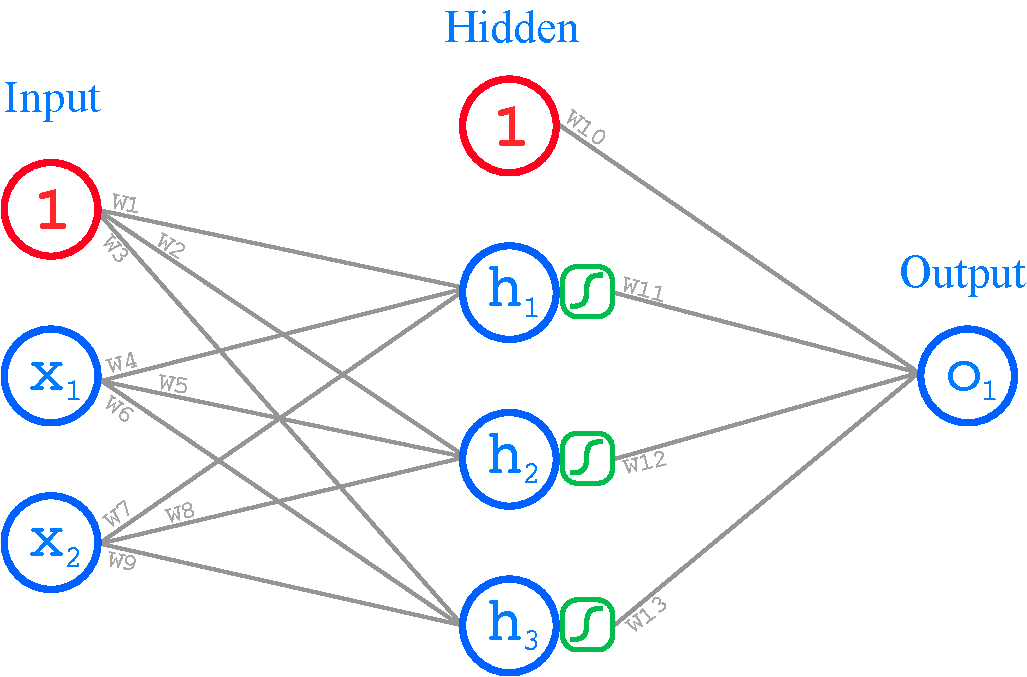
\includegraphics[width=0.7\textwidth]{figures/q1_neural_network.pdf}
  \caption{Diagram of the neural network containing two inputs, single hidden layer with three nodes and a single output layer.}
  \label{q1_network_diagram}
\end{figure}


\subsection*{Removing sigmoid from output layer}

In Lecture 13 example code (\url{http://astrowizici.st/teaching/phs5000/13/}), I removed the sigmoid for the output node (replacing it with $f(x) = x$). The reason I removed the sigmoid is the following. The output of the sigmoid is between 0 and 1, and this is used as predicted value from our model. However, in the loss function, we are comparing the predicted values with real values. The problem is that real value sometime outside the $[0, 1]$ range because they are normalized with mean $0$ and standard deviation of $1$. Consequently, the loss function will never approach zero. More importantly, the output of the model can not be used to generate the data.

I compare the loss function of the original and the modified models on \autoref{q1_lecture13_loss_compare}. We can see the modified model converges faster. The original will never converge to zero, even if we increase the number of interations.

\begin{figure}[!ht]
  \centering
  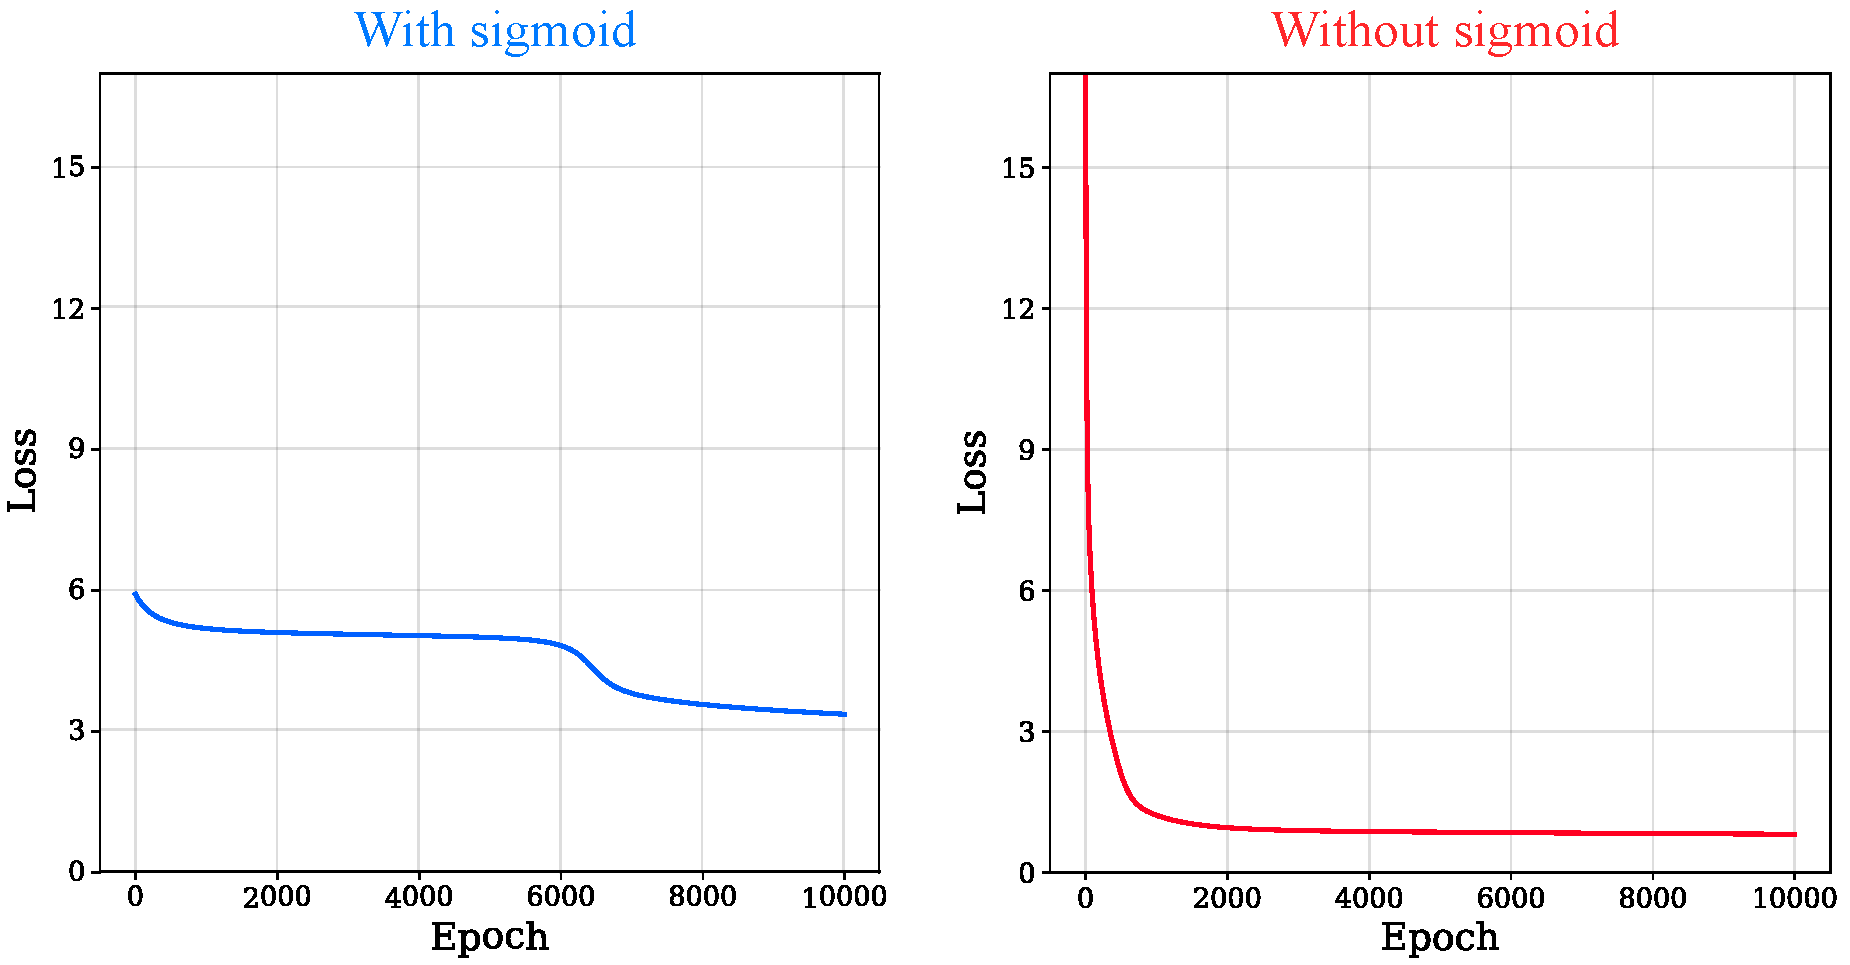
\includegraphics[width=1\textwidth]{figures/lecture13_loss_compared.pdf}
  \caption{Loss function for neural network from Lecture 13. The original code (left) contains sigmoid activation function in the output node, while the modified code (right) has no activation function ($f(x) = x$) in the output node. Both codes are otherwise identical, including the same seeding of random number generators.}
  \label{q1_lecture13_loss_compare}
\end{figure}

Original code: \\ \url{https://github.com/evgenyneu/ASP5020_data_analysis_problem_sets/blob/master/ps5/code/lecture13_original_with_signoid_output.py}

Modified code without output sigmoid: \\ \url{https://github.com/evgenyneu/ASP5020_data_analysis_problem_sets/blob/master/ps5/code/lecture13_remove_sigmoid_from_output.py}





\end{document}
